\documentclass[border=5pt]{standalone}
\usepackage{tikz}
\usetikzlibrary{arrows.meta, 3d, perspective, calc}
\usepackage{amsmath}
\begin{document}
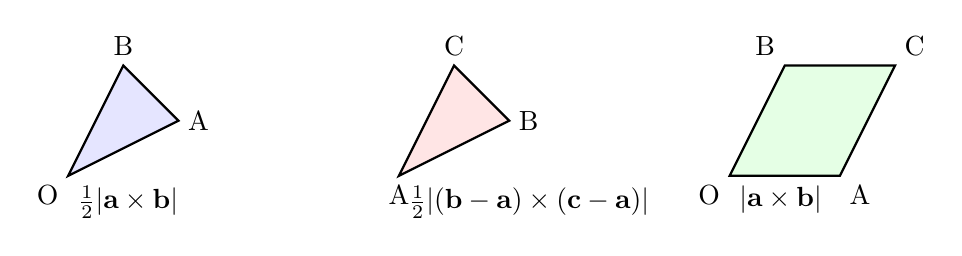
\begin{tikzpicture}[scale=0.7]
    % Triangle OAB
    \begin{scope}[shift={(-5,0)}]
        \draw[thick, fill=blue!10] (0,0) -- (2,1) -- (1,2) -- cycle;
        \node at (0,0) [below left] {O};
        \node at (2,1) [right] {A};
        \node at (1,2) [above] {B};
        \node[below right] at (0,0) {$\frac{1}{2}|\mathbf{a} \times \mathbf{b}|$};
    \end{scope}

    % Triangle ABC
    \begin{scope}[shift={(0,0)}]
        \draw[thick, fill=red!10] (1,0) -- (3,1) -- (2,2) -- cycle;
        \node at (1,0) [below] {A};
        \node at (3,1) [right] {B};
        \node at (2,2) [above] {C};
        \node[below right] at (1,0) {$\frac{1}{2}|(\mathbf{b}-\mathbf{a}) \times (\mathbf{c}-\mathbf{a})|$};
    \end{scope}

    % Parallelogram
    \begin{scope}[shift={(7,0)}]
        \draw[thick, fill=green!10] (0,0) -- (2,0) -- (3,2) -- (1,2) -- cycle;
        \node at (0,0) [below left] {O};
        \node at (2,0) [below right] {A};
        \node at (3,2) [above right] {C};
        \node at (1,2) [above left] {B};
        \node[below right] at (0,0) {$|\mathbf{a} \times \mathbf{b}|$};
    \end{scope}
\end{tikzpicture}
\end{document}
